%----------------------------------------------------------------------------------------
%	PREÁMBULO
%----------------------------------------------------------------------------------------

\documentclass[11pt, oneside]{book}
\usepackage[paperwidth=17cm, paperheight=22.5cm, bottom=2.5cm, right=2.5cm]{geometry}

% El borde inferior puede parecerles muy amplio a la vista. Les recomiendo hacer una prueba de impresión antes para ajustarlo

\usepackage{amssymb,amsmath,amsthm} % Símbolos matemáticos
\usepackage[spanish]{babel}
\usepackage[utf8]{inputenc} % Acentos y otros símbolos 
\usepackage{enumerate}
\usepackage{hyperref} % Hipervínculos en el índice
\usepackage{graphicx}
%\usepackage{subfig} % Subfiguras
\graphicspath{{Imagenes/}} % En qué carpeta están las imágenes

% Para eliminar guiones y justificar texto
\tolerance=1
\emergencystretch=\maxdimen
\hyphenpenalty=10000
\hbadness=10000

\linespread{1.25} % Asemeja el interlineado 1.5 de Word

\let\oldfootnote\footnote % Deja espacio entre el número del pie de página y el inicio del texto
\renewcommand\footnote[1]{%
\oldfootnote{\hspace{0.05mm}#1}}

\renewcommand{\thefootnote} {\textcolor{Black}{\arabic{footnote}}} % Súperindice a color negro

\setlength{\footnotesep}{0.75\baselineskip} % Espaciado entre notas al pie

\usepackage{fnpos} % Footnotes al final de pág.

\usepackage[justification=centering, font=bf, labelsep=period, skip=5pt]{caption} % Centrar captions de tablas y ponerlas en negritas

\newcommand{\imagesource}[1]{{\footnotesize Fuente: #1}}

\usepackage{tabularx} % Big tables
\usepackage{graphicx}
\usepackage{adjustbox}
\usepackage{longtable}

\usepackage{float} % Float tables

\usepackage[usenames,dvipsnames]{xcolor} % Color

\usepackage{pgfplots} % Gráficas
\pgfplotsset{compat=newest}
\pgfplotsset{width=7.5cm}
\pgfkeys{/pgf/number format/1000 sep={}}

\begin{document}

%----------------------------------------------------------------------------------------
%	PORTADA
%----------------------------------------------------------------------------------------

\title{ JUGADOR ARTIFICIAL DE DOMINÓ BASADO EN MÉTODOS DE MONTE CARLO} % Con este nombre se guardará el proyecto en writeLaTex

\begin{titlepage}
\begin{center}

\textsc{\Large Instituto Tecnológico Autónomo de México}\\[2em]

%Figura
\begin{figure}[h]
\begin{center}

\includegraphics[scale=0.50]{itam_logo.png}
\end{center}
\end{figure}

% Pueden modificar el tamaño del logo cambiando la escala

\textbf{\LARGE JUGADOR ARTIFICIAL DE DOMINÓ BASADO EN MÉTODOS DE MONTE CARLO}\\[2em]

\textsc{\large Tesis}\\[1em]

\textsc{\large que para obtener el título de}\\[1em]

\textsc{\LARGE Ingeniero en Computación}\\[1em]

\textsc{\large Presenta}\\[1em]

\textsc{\LARGE Andrés Cruz y Vera}\\[1em]

\textsc{\large Asesora}\\[1em]

\textsc{\LARGE Dr. Marco Antonio Morales Aguirre}\\[2em]

% Asegúrense de escribir el nombre completo de su asesor

\end{center}

\vspace*{\fill}
\textsc{Ciudad de México \hspace*{\fill} 2020}

\end{titlepage}

%----------------------------------------------------------------------------------------
%	DECLARACIÓN
%----------------------------------------------------------------------------------------

\thispagestyle{empty}

\vspace*{\fill}
\begingroup

\noindent
«Con fundamento en los artículos 21 y 27 de la Ley Federal del Derecho de Autor y como titular de los derechos moral y patrimonial de la obra titulada ``\textbf{Jugador articial de dominó basado en métodos de Monte Carlo}'', otorgo de manera gratuita y permanente al Instituto Tecnológico Autónomo de México y a la Biblioteca Raúl Bailléres Jr., la autorización para que fijen la obra en cualquier medio, incluido el electrónico, y la divulguen entre sus usuarios, profesores, estudiantes o terceras personas, sin que pueda percibir por tal divulgación una contraprestación.»

% Asegúrense de cambiar el título de su tesis en el párrafo anterior

\centering 

\vspace{5em}

\rule[1em]{20em}{0.5pt} % Línea para la fecha

\textsc{Fecha}
 
\vspace{8em}

\rule[1em]{20em}{0.5pt} % Línea para la firma

\textsc{Andrés Cruz y Vera}

\endgroup
\vspace*{\fill}

%----------------------------------------------------------------------------------------
%	DEDICATORIA
%----------------------------------------------------------------------------------------

\pagestyle{plain}
\frontmatter

\chapter*{}
\begin{flushright}
\textit{A mis padres,\\ por su incansable esfuerzo.}
\end{flushright}

%----------------------------------------------------------------------------------------
%	AGRADECIMIENTOS
%----------------------------------------------------------------------------------------

\chapter*{Agradecimientos}

\noindent Lorem ipsum dolor sit amet, consectetur adipiscing elit.

% Esta sección es lo único que la gente lee. True story :)

%----------------------------------------------------------------------------------------
%	RESUMEN
%----------------------------------------------------------------------------------------

% \chapter*{Resumen}

% \noindent El modelo de Solow afirma que el crecimiento de largo plazo se origina por un aumento en la productividad total de los factores. Romer agrega que esta productividad es generada por nuevas ideas. Las causas de la innovación son múltiples y en esta investigación se busca elucidar algunas de ellas. Desde una perspectiva heterodoxa que incluye resultados de la neurociencia o la genética, se argumenta que la confianza institucional, la inclusión social y la optimista percepción tecnológica tienen una relación positiva y significativa con la innovación. Entre las posibles razones causales está el hecho de que la confianza incentiva a los emprendedores por arriesgar, que la inclusión no limita el número de ideas potenciales en el mercado y que la optimista percepción es parte de las sociedades dinámicas que buscan innovar. Por el contrario, la intensidad religiosa guarda una relación negativa por la ausencia de actividad creativa que puede suscitar la interacción entre instituciones. La hipótesis se sostiene con un análisis econométrico de cincuenta y cinco países. La tesis cierra con el caso de estudio mexicano, en donde se propone que la etiología del lento crecimiento es la falta de innovación, la cual puede ser explicada por una baja confianza institucional y una alta religiosidad. El análisis está inmerso en la nueva globalización y la cuarta revolución tecnológica.

% \pagestyle{plain}

% \noindent 

%----------------------------------------------------------------------------------------
%	Summary
%----------------------------------------------------------------------------------------

% \chapter*{Summary}

% \noindent The Solow model states that long-term growth is caused by an increase in total factor productivity. Romer adds that this productivity is generated by new ideas. The causes of innovation are multiple and this research seeks to elucidate some of them. From a heterodox perspective that includes results from neuroscience or genetics, it is argued that institutional confidence, social inclusion and an optimistic technological perception have a positive and significant relationship with innovation. Among the possible causal reasons is the fact that confidence encourages entrepreneurs to take risks, that inclusion does not limit the number of potential ideas in the market and that an optimistic perception is part of the dynamic societies that innovate. On the contrary, religious intensity has a negative relationship due to the absence of creative activity that can arouse due to the interaction between institutions. The hypothesis is supported by an econometric analysis of fifty-five countries. The thesis closes with a case study on Mexico, where it is proposed that the etiology of its slow growth is the lack of innovation, which can be explained by low institutional confidence and high religiosity. The analysis is immersed in the new globalization and the fourth technological revolution.

% \pagestyle{plain}

% \noindent 

%----------------------------------------------------------------------------------------
%	TABLA DE CONTENIDOS
%---------------------------------------------------------------------------------------

\tableofcontents

%----------------------------------------------------------------------------------------
%	ÍNDICE DE CUADROS Y FIGURAS
%---------------------------------------------------------------------------------------

\listoftables

\listoffigures

%----------------------------------------------------------------------------------------
%	TESIS
%----------------------------------------------------------------------------------------

\mainmatter % Empieza la numeración de las páginas

\pagestyle{plain}

% Incluye los capítulos en el fólder de capítulos

\chapter*{Introducción}
\addcontentsline{toc}{chapter}{Introducción}

% La introducción no cuenta como primer capítulo

\noindent 

En el primer capítulo se presentará el problema que se aborda en este trabajo. Se dará el 
contexto histórico de la relación entre los videojuegos y los jugadores artificiales para luego 
identificar el problema y definir tanto los objetivos como la metodología a seguir.

\section{Contexto}

La historia de los juegos por computadora inicia desde la década de 1950 en el ámbito 
académico y en los años setenta y ochenta gana popularidad para el público en general. Los 
videojuegos han tenido un gran impacto en la cultura popular, así como en grandes figuras 
de la computación que tuvieron su primer acercamiento a los ordenadores por medio de 
estos y del lenguaje BASIC

Asimismo, los juegos de mesa han tenido un papel importante en el desarrollo del área de 
inteligencia artificial siendo una área muy fructífera de investigación como en el caso del 
ajedrez y la famosa contienda entre Deep Blue y Garry Kasparov

\subsection{Identificación del problema}

 El desarrollo de videojuegos es un ámbito multidisciplinario en donde se utilizan técnicas 
de inteligencia artificial para complementar la experiencia de juego del usuario. Los 
jugadores artificiales (o bots) cumplen un papel importante como contrincantes o 
personajes secundarios dentro del juego. 

Con miras a desarrollar una versión online del juego de dominó con un modelo de 
monetización basado en anuncios, se tiene como uno de los objetivo maximizar el número 
de impresiones de los anuncios en el usuario. Así, es necesario proveer una experiencia 
atractiva que tenga como efecto que el usuario pase un largo tiempo activo en la página.

El lanzamiento a mercado de un juego multijugador online presenta distintos retos. Entre 
ellos, existe la necesidad de crear una base mínima de usuarios que permita tener un tiempo 
razonable de espera para poder encontrar una partida a la cual unirse. Una forma de 
solventar parcialmente este obstáculo, particularmente en las primeras fases del 
lanzamiento, es contar con jugadores artificiales que suplementen la falta de contrincantes 
humanos.

Así, es deseable contar con un jugador artificial que permita a los usuarios iniciar una 
partida aun en las circunstancias en que no cuenten con suficientes personas para completar 
los equipos. Al momento en que se realiza este escrito, no se ha encontrado una 
implementación de código abierto de un jugador artificial para el juego de dominó (con las 
reglas que se usan en latinoamérica) que cuente tanto con una licencia que permita su uso 
comercial así como una interfaz de programación diseñada para su integración a un juego 
de tiempo real con usuarios humanos.



\subsection{Objetivos}

Implementar un programa de computadora que sea capaz de jugar en una partida de dominó 
como parte de un equipo de dos participantes que compiten con dos contrincantes.

\subsection{Metodología}

Para la implementación del bot, se decidió utilizar la metodología de cascada debido a que 
el alcance y la funcionalidad del proyecto es relativamente pequeña.

\subsection{Organización del documento}
\begin{enumerate}
    \item Introducción
    \item Análisis de requisitos del software
    \item El juego de dominó
    \item Diseño del programa
    \item Implementación
    \item Validación
    \item Conclusiones
\end{enumerate}


% Se sugiere que el primer párrafo de cada sección no tenga sangría: \noindent


\chapter{Análisis}

\noindent
Una vez que se ha identificado el problema, se formulará una primera
aproximación a la solución por medio de los requerimientos funcionales que debe
cumplir, así como por las restricciones que debe satisfacer. También se
mostrarán trabajos relacionados.

\newpage

\section{Requerimientos funcionales}

El sistema generará una jugada a partir del estado actual del juego. Es decir,
el progama recibirá como entrada una representación de sus fichas asignadas así
como de las fichas tiradas por los otros participantes y como salida indicará
cual de sus fichas debe jugarse. También será posible elegir distintos niveles
de juego para el programa

\section{Requerimientos no funcionales}

El programa debe generar las jugadas en un tiempo razonable. Debe siempre
terminar la ejecución antes de un lapso predeterminado para poder utilizarse en
un juego de tiempo real contra contrincantes humanos y no debe poseer
información sobre las manos de sus contrincantes ni de su pareja de equipo.

En segundo lugar, el desempeño del programa tiene que ser mejor que la
estrategia más sencilla posible (el jugador greedy): de entre las fichas que se
tiene en la mano, siempre bajar la de mayor puntaje. Una jugada greedy es
sumamente barata de calcular. De no cumplirse con este requisito no tendría
sentido utilizar una estrategía más compleja y costosa en tiempo y recursos
computacionales.

Así, se pone como meta que un equipo de jugadores artificiales debe vencer a un
equipo de jugadores greedy en al menos 70\% de las partidas. Se considera que
este margen es el minimo para justificar el uso de un algoritmo distinto a la
estrategía greedy.

Por último, debe exponer una API sencilla para ser integrado a distintas
interfaces, tanto aplicaciones web como móviles.

\section{Restricciones}

El software a desarrollar cuenta con dos restricciones principales. En primer
lugar, en cuanto a los recursos para implementar la solucion, se cuenta con un
periodo aproximado de 6 meses para completar el desarrollo del sistema así como
de un solo desarrollador (el autor de este trabajo).

En segundo lugar, el sistema debe cumplir con los requerimientos funcionales y
no funcionales dentro de un ambiente de ejecución en la nube con un costo
razonable. Es dificil estimar el costo de los recursos computacionales que
consumirá la solución, pues depende de la cantidad de usuarios del sistema así
como de su comportamiento de uso. No se cuenta con los datos necesarios para
estimar la naturaleza de la carga a la que el sistema debe hacer frente pero se
puede definir unas caracteristicas mínimas del ambiente de ejecución en el cual
la solución debe correr.

Como un punto de referencia, se ha elegido la instancia más modesta de la
categoría de servidores de proposito general de Digital Ocean. Dicho servidor
cuenta con ocho gigabytes de memoria RAM y con dos procesadores virtuales. La
máquina virtual corre sobre procesadores Intel Xeon Skylake con una velocidad
base de 2.7 ghz y con máxima velocidad de 3.7 ghz. El costo del servidor es de
sesenta dólares al mes. Se eligió Digital Ocean por los creditos que regala para
probar los servidores.

Si el sistema no puede correr en un servidor de esta naturaleza, es muy probable
que en una escala más grande el costo de la solución sea prohibitivo para su
uso.

\section{Trabajos relacionados}

Uno de los trabajos importante en el ambito de algoritmos  para juegos de
información imperfecta lo realiza Ginsberg  (2001).  Con esta metodología logra
implementar un jugador de Bridge de nivel experto.

Por otra parte, un jugador artificial en un contexto de incertidumbre puede
estudiarse desde la perspectiva de procesos de decisión de markov como en la
disciplina de aprendizaje por refuerzo. En este campo es importante el trabajo
de Mnih et al. (2013) que es uno de los primeros en integrar aprendizaje
profundo a los algoritmos de aprendizaje por refuerzo para la creación de
agentes en el juego de atari.

Long et al. (2010) realizaron un trabajo en donde , a partir de árboles de juego
sintéticos, definen indicadores estadísticos que les permiten identificar
propiedades importantes de juegos de información imperfecta en los que el método
de Perfect Information Monte Carlo (PIMC)  se puede adaptar exitosamente. Dicho
trabajo extiende la línea de investigación sobre las limitaciones de PIMC en el
contexto de información imperfecta que inician Frank y Basin (1998)

Asimismo, se recuperó de la web un proyecto de licenciatura sobre un jugador
artificial para dominó (en el texto se le refiere como Latin-American dominoes)
desarrollado por Angeris y Li (2016) de la universidad de Stanford. El proyecto
consiste en simulaciones para contrastar distintas algoritmos pero no tiene la
finalidad de ser consumido como una API.
% La siguiente gráfica está hecha a mano porque la que arroja R se pixelea un poco al importarla a LaTeX. Pueden apoyarse en Excel para obtener las coordenadas más rápido

% \begin{figure}[H]
% \begin{center}
% \caption{PIB mundial de los últimos dos milenios}
% \label{PIB_MUN}
% \begin{tikzpicture}
% \begin{axis}[
%     xlabel={Año},
%     ylabel={PIB (billones)},
%     xtick pos=left,
%     ytick pos=left,
%     xtick={500,1000,1500,2000},
%     ytick={0,50,100},
%     scale only axis=true,
%     width=0.6\textwidth,
%     height=0.4\textwidth,
% ]

% \addplot[
%     color=red,
%     ]
%     coordinates {
%     (1,0)(1000,0)(1500,0)(1600,1)(1700,1)(1820,1)(1870,2)(1900,3)(1913,5)(1940,8)(1950,9)(1951,10)(1952,10)(1953,11)(1954,11)(1955,12)(1956,12)(1957,13)(1958,13)(1959,14)(1960,15)(1961,15)(1962,16)(1963,17)(1964,18)(1965,19)(1966,20)(1967,20)(1968,22)(1969,23)(1970,24)(1971,25)(1972,26)(1973,28)(1974,28)(1975,29)(1976,30)(1977,31)(1978,33)(1979,34)(1980,35)(1981,35)(1982,36)(1983,37)(1984,38)(1985,40)(1986,41)(1987,43)(1988,45)(1989,46)(1990,47)(1991,48)(1992,48)(1993,49)(1994,51)(1995,53)(1996,55)(1997,57)(1998,58)(1999,60)(2000,63)(2001,65)(2002,66)(2003,69)(2004,73)(2005,76)(2006,80)(2007,85)(2008,87)(2009,87)(2010,91)(2011,95)(2012,98)(2013,101)(2014,105)(2015,108)
%     };

% \end{axis}
% \end{tikzpicture}

% \imagesource{elaboración propia con datos de Maddison (2010) y el Banco Mundial.}
% \end{center}
% \end{figure}


\chapter{El juego de dominó}

\noindent

El dominó es un juego conocido alrededor de todo el mundo. Existen distintas
modalidades de juego que varian en el número de jugadores o en las reglas para
bajar una ficha. En esta sección se define el tipo de dominó del que trata este
trabajo. Posteriormente, se discuten algunas propiedades importantes del juego
que permiten hacer una estimación de su complejidad y compararlo con la
complejidad de otros juegos de mesa.

\newpage

\section{Dinámica del juego}

Para jugar se utilizan veintiocho fichas, cada una marcada con dos números entre
el cero y el seis. Al iniciar la partida, se revuelven aleatoriamente las fichas
y se reparten siete a cada uno de los cuatro jugadores. Los jugadores se dividen
en dos equipos y se encuentran sentados en circulo, de tal forma que no hay dos
jugadores del mismo equipo adyacentes.

El jugador con la ficha de dos seises es el primero en tirar y el orden de las
tiradas sigue a la derecha. En cada turno, el jugador puede bajar una ficha si
tiene algun número en común con los extremos externos de las fichas que ya se
han jugado. El objetivo del juego es ser el equipo con el primer jugador que ha
bajado todas sus fichas o, en caso de que ningún jugador pueda bajar fichas, ser
el equipo cuyas fichas sumen el menor número de puntos.

\section{Factor promedio de ramificación}

Uno de los componentes de la complejidad del juego es el número promedio de
acciones que cada jugador puede tomar en su turno, tambien conocido como factor
promedio de ramificación. Un cálculo analítico de este factor es dificil, pues
depende de la repartición aleatoria al inicio del juego así como de la
estrategia de cada jugador. Para obtener una estimación del factor se realizó la
simulación de diez mil juegos con dos equipos de jugadores greedy y se obtuvo
los siguientes resultados.

\begin{figure}[ht]
    \begin{center}
        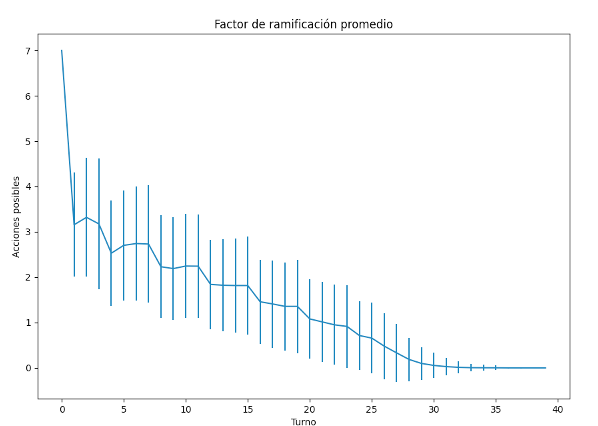
\includegraphics{factor_prom_ramificacion.png}
        \caption{Factor de ramificación promedio}
        \label{FPR}
    \end{center}
\end{figure}

En la figura \ref{FPR} se muestra, en el eje vertical, el número promedio de
fichas que un jugador puede tirar en el turno indicado en el eje horizontal. El
primer jugador siempre puede tirar cualquiera de sus fichas. Después de él, los
jugadores pueden tirar 3 o menos fichas en promedio. Este factor de ramificación
es pequeño si se compara al de otros juegos de mesa como el ajedrez, el cual
tiene un factor estimado entre 31 y 35 movimientos.

\section{Información imperfecta}

El segundo componente que influye en la complejidad del juego es la
incertidumbre asociada a las fichas que no se conocen. Para obtener una medida
de esta incertidumbre se calculó el número de configuraciones posibles de la
información escondida. Desde la perspectiva del primer jugador en tirar y
suponiendo que todos los jugadores bajan una ficha, se puede calcular el número
de formas distintas en que se pueden repartir las fichas que no se conocen para
cada vuelta del juego (cada vez que vuelve a ser turno del primer jugador ) y se
obtuvo la siguiente tabla.

\begin{table}[H]
    \centering
    \caption{Posibles configuraciones de las fichas que no se conocen}
    \label{PC}
    \begin{tabular}{|c|c|}
        \hline
        Vuelta & Posibles formas de repartir las fichas desconocidas \\
        \hline
        1      & 400 millones                                        \\
        2      & 17 millones                                         \\
        3      & 750 mil                                             \\
        4      & 34 mil                                              \\
        5      & 1600                                                \\
        6      & 90                                                  \\
        7      & 6                                                   \\
        \hline
    \end{tabular}

    % \begin{tabular}{c}
    % \footnotesize{Fuente: Bojilov y Phelps (2012).}
    % \end{tabular}

\end{table}

Tomando en cuanta ambos componentes de la complejidad, se concluye que la
incertidumbre asociada a la información imperfecta en las primeras vueltas del
juego muestra ser el mayor reto a superar.

% \subsection{Cambios cerebrales y genéticos}

% \noindent Brizendine (2010) escribe que algunos científicos piensan que ciertas áreas del cerebro son como centros de actividad que mandan señales eléctricas a otras áreas del cerebro ocasionando un determinado comportamiento.\footnote{ Por ejemplo, en el hombre la corteza del cíngulo anterior pesa opciones, detecta conflicto y motiva decisiones. La unión temporoparietal busca soluciones rápidas y ante situaciones estresantes toma en cuenta la perspectiva de otros individuos. La corteza cingulada anterior rostral se encarga de procesar los errores sociales, como la aprobación o desaprobación de otros.}

% \begin{quote}
%     \small{Mientras que la distinción entre los cerebros de niños y niñas empieza biológicamente, estudios recientes muestran que es \textit{solo} el comienzo. La estructura cerebral no está escrita sobre piedra en el nacimiento ni al final de la infancia, como antes se creía, sino que continúa cambiando a lo largo de la vida. Más que ser inmutable, nuestros cerebros son mucho más plásticos y cambiables de lo que los científicos creían hace una década. El cerebro humano es también la máquina de aprendizaje más talentosa que conocemos. Así que nuestra cultura y el cómo nos enseñaron a comportarnos desempeñan un papel importante en el diseño y reestructura de nuestros cerebros (Brizendine 2010, 5-6).}
% \end{quote}

% % Para citas muy largas es mejor el \begin{quote}

% \vspace{1em}
% \noindent \textbf{Hipótesis 3.} \hfill\begin{minipage}{\dimexpr\textwidth-3cm}
% \textit{La intensidad religiosa está relacionada negativamente con la innovación.}
% \end{minipage}
% \vspace{1em}

% Para plantear hipótesis


% Para diseñar tablas


\chapter{Modelo econométrico}

\noindent Este capítulo tiene el propósito de probar empíricamente las hipótesis planteadas previamente y está dividido en dos secciones.

\newpage

\section{Regresión lineal múltiple}

\subsection{Modelo y resultados}

\noindent Ulteriormente, se corrió una regresión lineal múltiple en la que la variable dependiente es la innovación y las variables independientes son los cuatro índices construidos: 
 
\begin{equation}
   Y = \beta_{0} + \beta_{1} X_{i1} + \beta_{2} X_{i2} + \beta_{3} X_{i3} + \beta_{4} X_{i4} +\varepsilon, \label{1}
\end{equation}

% Para escribir ecuaciones

\begin{table}[H]
\centering
\caption{Resultados del modelo econométrico}
\label{REG}
\begin{tabular}{|ccccc|}
  \hline
 & Estimador & Desv. est. & Valor $t$ & Pr($>|t|$) \\ 
  \hline
  $\alpha$ & x & x & x & x \\ 
  CI & x & x & x & x \\ 
  IS & x & x & x & x \\ 
  IR & x & x & x & x \\ 
  PT & x & x & x & x \\ 
   \hline
\multicolumn{5}{|c|}{Error est. de res. = x con x gr. de libertad}
    \\
    \multicolumn{5}{|c|}{$R^2$ = x y $\bar{R}^2$ = x}
 \\
 \multicolumn{5}{|c|}{Estadístico $F$ = x, con un valor $p$ = x }
      \\
\hline
\end{tabular}

\end{table}


\chapter{El caso mexicano}

\noindent En este último capítulo se analiza el caso mexicano en dos partes: la dimensión nacional y la internacional. 

\newpage

\section{Dimensión nacional}

\subsection{¿Por qué no crecemos?}

\noindent El Grupo Huatusco se ha reunido por más de quince años intentando responder la pregunta de por qué México no crece a mayores tasas.

\begin{figure}[H]
\begin{center}
\caption{Brecha entre productividad y remuneración laboral en el mundo (1948-2016)}
\label{PROD_W}
\begin{tikzpicture}
\begin{axis}[
    xlabel={Año},
    ylabel={Cambio porcentual acumulado},
    xtick pos=left,
    ytick pos=left,
    xtick={1950,1970,1990,2010},
    ytick={0,125,250},
    scale only axis=true,
    width=0.6\textwidth,
    height=0.4\textwidth,
]

\addplot[
    color=red,
    ]
    coordinates {(1948,0)
(1949,1.5)
(1950,9.3)
(1951,12.4)
(1952,15.6)
(1953,19.5)
(1954,21.6)
(1955,26.5)
(1956,26.7)
(1957,30.1)
(1958,32.8)
(1959,37.6)
(1960,40)
(1961,44.4)
(1962,49.8)
(1963,55)
(1964,60)
(1965,64.9)
(1966,70)
(1967,72.1)
(1968,77.2)
(1969,77.9)
(1970,80.4)
(1971,87.1)
(1972,92)
(1973,96.7)
(1974,93.7)
(1975,97.9)
(1976,103.4)
(1977,105.8)
(1978,107.8)
(1979,108.1)
(1980,106.6)
(1981,111)
(1982,107.9)
(1983,114.1)
(1984,119.7)
(1985,123.4)
(1986,128)
(1987,129.1)
(1988,131.8)
(1989,133.7)
(1990,137)
(1991,138.9)
(1992,147.6)
(1993,148.4)
(1994,150.7)
(1995,150.9)
(1996,156.9)
(1997,160.5)
(1998,165.7)
(1999,172.1)
(2000,178.5)
(2001,182.8)
(2002,190.7)
(2003,200.2)
(2004,208.2)
(2005,213.6)
(2006,215.5)
(2007,217.7)
(2008,218.2)
(2009,224.7)
(2010,234.3)
(2011,234.7)
(2012,236.5)
(2013,237.6)
(2014,239.3)
(2015,241.1)
(2016,241.8)
    };
    
    \addplot[
    dashed,
    color=blue,
    ]
    coordinates {(1948,0)
(1949,6.3)
(1950,10.5)
(1951,11.8)
(1952,15)
(1953,20.8)
(1954,23.5)
(1955,28.7)
(1956,33.9)
(1957,37.1)
(1958,38.2)
(1959,42.6)
(1960,45.5)
(1961,48)
(1962,52.5)
(1963,55)
(1964,58.5)
(1965,62.5)
(1966,64.9)
(1967,66.9)
(1968,70.7)
(1969,74.7)
(1970,76.6)
(1971,82)
(1972,91.3)
(1973,91.3)
(1974,87)
(1975,86.9)
(1976,89.7)
(1977,93.1)
(1978,96)
(1979,93.5)
(1980,88.6)
(1981,87.6)
(1982,87.8)
(1983,88.4)
(1984,87)
(1985,86.3)
(1986,87.3)
(1987,84.6)
(1988,83.9)
(1989,83.7)
(1990,82.2)
(1991,81.9)
(1992,83.1)
(1993,83.4)
(1994,83.8)
(1995,82.7)
(1996,82.8)
(1997,84.8)
(1998,89.2)
(1999,91.9)
(2000,92.9)
(2001,95.6)
(2002,99.4)
(2003,101.7)
(2004,100.9)
(2005,100.1)
(2006,100.2)
(2007,101.7)
(2008,101.7)
(2009,109.7)
(2010,111.6)
(2011,109.1)
(2012,107.3)
(2013,108.3)
(2014,109.2)
(2015,112.8)
(2016,115.1)};
    
\end{axis}
\end{tikzpicture}

\imagesource{elaboración propia con datos del Economic Policy Institute.}
\end{center}
\end{figure}

% Gráfica con dos colores a mano


\chapter*{Conclusiones}
\addcontentsline{toc}{chapter}{Conclusiones}

% Las conclusiones tampoco cuentan como capítulo

\noindent Hegel (1953) escribe en su obra \textit{Lecciones sobre la filosofía de la Historia Universal} un par de conceptos que son útiles para comprender de manera abstracta la esencia detrás de esta investigación.


%----------------------------------------------------------------------------------------
%	APÉNDICES
%----------------------------------------------------------------------------------------

\begin{appendix}

\chapter{Cuadros anexos}

\noindent 

\end{appendix}

%----------------------------------------------------------------------------------------
%	BIBLIOGRAFÍA
%----------------------------------------------------------------------------------------


\chapter*{Referencias}
\addcontentsline{toc}{chapter}{Referencias}

% Macro. Esto es muy importante, no lo borren

\makeatletter
\renewenvironment{thebibliography}[1]
     {\@mkboth{\MakeUppercase\refname}{\MakeUppercase\refname}%
      \list{}%
           {\setlength{\labelwidth}{0pt}%
            \setlength{\labelsep}{0pt}%
            \setlength{\leftmargin}{\parindent}%
            \setlength{\itemindent}{-\parindent}%
            \@openbib@code
            \usecounter{enumiv}}%
      \sloppy
      \clubpenalty4000
      \@clubpenalty \clubpenalty
      \widowpenalty4000%
      \sfcode`\.\@m}
     {\def\@noitemerr
       {\@latex@warning{Empty `thebibliography' environment}}%
      \endlist}
\makeatother

\begin{thebibliography}{111}

% Lista

% La manera recomendada para citar papers o libros en el formato de Chicago esta en el siguiente vínculo: https://www.chicagomanualofstyle.org/tools_citationguide/citation-guide-2.html

% Es importante poner el apellido del autor seguido del año de publicación, una coma y las páginas consultadas en el texto antes de puntuar y entre paréntesis para las citas en el cuerpo de la tesis

% Ejemplo:

% Las \textit{causas próximas} del crecimiento son conocidas: tecnología, capital humano y físico. La pregunta es ¿por qué unos países sí tienen estas causas próximas y otros no? La respuesta son las \textit{causas fundamentales:} suerte, geografía, cultura e instituciones (Acemoglu 2009, 110).

%AAAAA
\bibitem{abram57} Abramovitz, Moses. 1957. «Resources on Output Trends in the United States since 1870.» \textit{The American Economic Review} 46 (2): 5–23.

\bibitem{acemoglu09} Acemoglu, Daron. 2009. \textit{Introduction to Modern Economic Growth.} Princeton: Princeton University Press.

%BBBBB

%CCCCC

%DDDDD

%EEEEE

%FFFFF

%GGGGG

%HHHHH

%IIIII

%JJJJJ

%KKKKK

%LLLLL

%MMMMM

%NNNNN

%OOOOO

%PPPPP

%QQQQQ

%RRRRR

%SSSSS

%TTTTT

%UUUUU

%VVVVV

%WWWWW

%XXXXX

%YYYYY

%ZZZZZ

\end{thebibliography}

\newpage
\thispagestyle{empty}
\begin{table}[p]
\centering
\small
\label{ed}
\begin{tabular}{c}
\textit{Confianza institucional, inclusión social,}\\ \textit{intensidad religiosa y percepción}\\ \textit{tecnológica como factores de innovación}\\ \textit{para el crecimiento económico,}\\ escrito por Farid Hannan,\\ se terminó de imprimir en diciembre de 2018\\ en los talleres de Tesis Matozo.\\ Campeche 156, colonia Roma,\\ Ciudad de México.
\end{tabular}
\end{table}

% Si lo prefieren, avisen a su taller que esta página ya la incluyeron ustedes para que no les impriman las que ellos usan. Lo recomiendo ampliamente

%%%%%%%%%%%%%%%%%%%%%%%%%%%%%%%%%%%%%%%%%%%%%%%%%%%%%%%%%%%%%%%%%%%%%%%%%%%%%%%%%%%%%%%

\end{document}